\documentclass[a4paper, 12pt]{article}
\usepackage{listings} 
\usepackage{xcolor}
\usepackage{mdframed}
\usepackage{graphicx}
\definecolor{code-gray}{gray}{0.93}
\begin{document}
\title{ECE 341 - Lab \#4}
\author{Collin Heist}
\date{\today}
\maketitle
\pagenumbering{roman}
\tableofcontents
\lstlistoflistings
\newpage
\pagenumbering{arabic}

\section{Introduction}
The purpose of this lab is to introduce the concepts of interrupt-driven programming with C. The general design of this lab is nearly identical to that of Lab \#3, except rather than using a fixed RPM and having our one millisecond delay function implemented using only software, we'll be using a one millisecond interrupt and a variable RPM.

As previously stated, this lab is largely the same as Lab \#3. Thanks to this, my preliminary plan worked just as planned. We'll once again be implementing a software-based finite state machine, where the transitions are controlled by the current state, and the buttons being pressed. The largest change is that rather than one simple \textbf{while(1)} loop that sequentially checks the buttons, decodes them, outputs to the motor, and then waits, we'll be reading the buttons at a fixed interval, and outputting to the motor at a preset interval as well (based on the button delay). The main loop will cycle every (approximately) one millisecond, and decrement the respective counters for the above-listed tasks.

\section{Implementation}
The system initialization function needed only one change, and that is the implementation of opening \textbf{Timer 1}. The function is shown below:

	\begin{mdframed}[backgroundcolor=code-gray, roundcorner=10pt,
								innerleftmargin=5, innertopmargin=5, innerbottommargin=5]	
	\begin{lstlisting}[language=C, caption=System Initialization, tabsize=2]
	void system_init(void) {
		Cerebot_mx7cK_setup();
		OpenTimer1(T1_ON | T1_PS_1_1, T1_TICK-1);
		PORTSetPinsDigitalIn(IOPORT_G, BTN1 | BTN2);
		PORTSetPinsDigitalOut(IOPORT_B, SM_COILS |
			BIT_2 | BIT_3 | BIT_4);
		LATBCLR =  SM_COILS | BIT_2 | BIT_3 | BIT_4;
	}
	\end{lstlisting}
	\end{mdframed}
	
This line turns on Timer 1, sets its pre-scale value to 1, and then sets its period to 1ms. The rest of this code is nearly identical to last week's lab. The provided handout says to open \textit{only} bits 2, 3, 4, 7, 8, 9, and 10 as outputs (hence the long opening statement).

The next function that needed to be changed was \textbf{decode\_buttons()}, as the control modes that each combination of buttons represents has changed. The new button configurations are as follows:

\begin{table}[ht]
\centering
\begin{tabular}{cc|ccc|c}
\multicolumn{2}{c}{\textbf{Inputs}} & \multicolumn{3}{c}{\textbf{Control Modes}} & \textbf{Output}\\
\hline
Button 2 & Button 1 & Direction & Step Mode & Speed (RPM) & - \\
\hline
Off & Off & CW & HS & 15 & 0b0100 \\
Off & On & CW & FS & 15 & 0b0101 \\
On & Off & CCW & HS & 10 & 0b0010 \\
On & On & CCW & FS & 25 & 0b1011 \\
\end{tabular}
\caption{New Stepper Motor Control Modes}
\end{table}

The benefit of this new control scheme is that button one and two directly control the step mode and direction directly. The downside is that the new \textbf{decode\_buttons()} function has to also return an encoded speed. Rather than returning a shifted value of the delay itself, I chose to simply have 10ms, 15ms, and 25ms represent  0, 1, and 2 respectively. This implementation is shown below, in Listing 2:

	\begin{mdframed}[backgroundcolor=code-gray, roundcorner=10pt,
								innerleftmargin=5, innertopmargin=5, innerbottommargin=5]	
	\begin{lstlisting}[language=C, caption=Button Decoding, tabsize=2]
	unsigned int decode_buttons(unsigned int portG) {
		unsigned int buttons = portG >> 6;
		// 00 -> 0100, 01 -> 0101, 10 -> 0010, 11 -> 1011
		return (buttons < 2 ? 4 + buttons :
			((buttons & 1) << 3) + buttons);
	}
	\end{lstlisting}
	\end{mdframed}
	
Although this function might look confusing at first, it is quite simple. First, it bit-shifts down the return from \textbf{read\_buttons()} (which hasn't changed at all) so that both buttons are in bits 0 and 1. Then, because \textbf{BTN1} and \textbf{BTN2} both directly correspond to the direction and step mode of the motor, the only 'computation' necessary is the speed. So, the return is calculated by adding the value of buttons with the correct time.

The stepper motor's state machine function is identical to Lab \#3, with the only change being that the switch statement now ignores the upper two bits of the control mode by using a bit mask. This is done because the speed of the motor doesn't affect any of the state transitions.

The \textbf{output\_to\_stepper\_motor()} function was not changed at all from last week's lab. Given that we're using the same motor, and the state outputs are identical to last week, there was no need to adjust this code.

This next function essentially replaces last lab's two functions \textbf{sw\_delay()} and \textbf{delayMS()}. The code is shown below:

	\begin{mdframed}[backgroundcolor=code-gray, roundcorner=10pt,
								innerleftmargin=5, innertopmargin=5, innerbottommargin=5]	
	\begin{lstlisting}[language=C, caption=One Millisecond Timer Loop, tabsize=2]
	void Timer1_delay(unsigned int* button_delay,
		unsigned int* step_delay) {
		while (!mT1GetIntFlag()) {}
		mT1ClearIntFlag();	
		LATBINV = LEDA;

		*step_delay -= 1;
		*button_delay -= 1;
	}
	\end{lstlisting}
	\end{mdframed}
	
This function performs two primary operations; it waits one millisecond for the interrupt flag from Timer 1 to trigger, and then decrements the provided variables. As configured back in \textbf{system\_init()}, Timer 1 triggers the T1 interrupt flag every one millisecond. So once the function is entered, the infinite while loop waits for flag, then resets it to turn the flag back on. \textbf{LEDA} is toggled for verifying the function's operation using an oscilloscope. Because the two variables are passed in as pointers, their values can be changed once they're de-referenced. Their values are reduced by one to signify one millisecond has passed.

The reason for using \textbf{unsigned int} variables rather than just \textbf{int} for the two delay parameters is because it provided a greater range of delay to the function. During the normal operation of this program, each of these respective delay variables will never be decremented below zero. This is because they're reset to their initial values as soon as they become zero. Because of this, casting them as unsigned rather than signed gives twice the maximum delay for each of them (not that it matters in this specific case). 

The implementation of all of the above-listed functions is in the program's main function, that is essentially broken into two parts: the variable initialization and the infinite while loop.

	\begin{mdframed}[backgroundcolor=code-gray, roundcorner=10pt,
								innerleftmargin=5, innertopmargin=5, innerbottommargin=5]	
	\begin{lstlisting}[language=C, caption=Main Variable Initialization, tabsize=2]
	int main() {
		system_init();
		unsigned int button_delay  = BTN_PRD;
		unsigned int step_delay    = MOT_PRD;
		unsigned int rev_min       = 10;
		unsigned int del_mode      = 0;
		unsigned int button_status = 0;
		unsigned int control_mode  = 0;
		unsigned int motor_hex     = 0;
		...
	\end{lstlisting}
	\end{mdframed}
	
As discussed before, the variables are all \textbf{unsigned int} to give a higher maximum value for the delays. As for why the button, control, and hexcode variables are unsigned is simply because there is never a situation where they'll logically \textit{need} to be a negative number, so to remain consistent and possibly eliminate bugs, I stuck with unsigned throughout my code.

I chose to have delay variables start at their delay values and move towards zero for two reasons: it makes more logical sense (to me at least) as a value of how \textit{long is left} in each cycle, and for how the end-of-period detection is implemented.

The initial value of the delay variables is defined in the header file for this lab. I did not change anything in this header file except for the addition of a few macros, shown here:

	\begin{mdframed}[backgroundcolor=code-gray, roundcorner=10pt,
								innerleftmargin=5, innertopmargin=5, innerbottommargin=5]	
	\begin{lstlisting}[language=C, caption=Header File Macros, tabsize=2]
	#ifndef __LAB3_H__
		#define __LAB3_H__
		...
		#define T1_SCALE			1
		#define TOGG_PER_SEC	1000
		#define T1_TICK				(FPB/T1_SCALE/TOGG_PER_SEC)
		
		#define BTN_PRD				100
		#define MOT_PRD				10

		#define RPM10					0
		#define RPM15					1
		#define RPM25					2
	#endif
	\end{lstlisting}
	\end{mdframed}
	
The second set are just the initial values of both delay loops. The buttons are supposed to be sampled every 100 ms (as stated in the lab handout), and I chose a value of 10 for the motor somewhat arbitrarily, but it is the timing used when neither buttons are pressed (so a somewhat neutral state). The implementation of the final three macros is shown below as a part of the second part of the main function, the infinite loop:

	\begin{mdframed}[backgroundcolor=code-gray, roundcorner=10pt,
								innerleftmargin=5, innertopmargin=5, innerbottommargin=5]	
	\begin{lstlisting}[language=C, caption=Infinite Program Loop, tabsize=2]
	...	
	while (1) {
		if (!button_delay) {
			button_status = read_buttons();
			control_mode  = decode_buttons(button_status);

			button_delay  = BTN_PRD;
			LATBINV       = LEDB;
		}

		if (!step_delay) {
			motor_hex = stepper_state_machine(control_mode);
			output_to_stepper_motor(motor_hex);

			// Look at bits 2-3 for the proper time delay
			del_mode = (control_mode & 12) >> 2;
			rev_min  = (del_mode == RPM10) ? 10 :
				(del_mode == RPM15) ? 15 : 25;
			step_delay = 1.0 / 
				((float)rev_min * 100.0 / 60.0 / 1000.0);
            
			LATBINV  = LEDC;
		}
		Timer1_delay(&button_delay, &step_delay);
	}
    
	return 0;	// End of main()
	\end{lstlisting}
	\end{mdframed}
	
This loop implements all the above functions. The first \textbf{if} statement checks if the button delay is a non-zero number, and if it \textit{isn't} non-zero, then the buttons are read, decoded, and then then the button delay is reset to 100. After toggling \textbf{LEDB}, the button section of the code is finished. 

The next \textbf{if} statement deals with the motor. Once again, if the delay counter is zero, the state machine is incremented to the appropriate next state, the output is sent to the motor, and then the delay is reset. The delay's reset value is dependent upon the current control mode, because each case of button presses corresponds to a different RPM of the motor. As stated earlier, bits 2 and 3 are the encoded RPM of the control mode, so the other bits are ignored, and then the predefined macros are used to check at which RPM the motor is. 

I could have used any other operator for checking if the delay had reset to zero, especially \textbf{==} or \textbf{<=}. I chose not to do this because there should never be a point where the delays are decremented to zero and \textit{not} reset immediately. If I had chosen to use one of those operators, I would have used the \textbf{<=} operator, because it works even in the case where the decrement to 0 was exactly missed (which should not possible). But, if I were to use that operator in this case where the value is reset \textit{to} the proper delay, I would need to change my variable types to \textbf{int}, not \textbf{unsigned int}. This is to prevent the value from underflowing to a very large number, if it is missed.

\section{Testing and Verification}
The testing for this lab is quite straightforward. Because of the requirement to toggle certain LED's every time an \textit{event} happens, by hooking up the oscilloscope's probes to the proper pins on the board, the period of the LED toggles can be verified (and thus, the code itself). Beyond the LED verification, it should be visually easy to determine if the RPM of the motor is slower or faster  than others, and the direction of the motor is also easy to visually verify.

My oscilloscope captures are attached in \textbf{Section 6}, and the timing should be compared with the following table:

\begin{table}[h]
\centering
\begin{tabular}{cc|cccc}
\multicolumn{2}{c|}{\textbf{Inputs}}  & \multicolumn{4}{c}{\textbf{Controls}} \\
\hline
BTN2 & BTN1 & Step Mode & RPM & Calc. Step Delay & Meas. Step Delay \\
\hline
Off & Off & HS & 15 & 40.000 ms & 40.000 ms \\
Off & On & FS & 15 & 40.000 ms & 40.000 ms \\
On & Off & HS & 10 &  60.000 ms & 60.096 ms \\
On & On & FS & 25 & 24.000 ms & 24.000 ms\\
\end{tabular}
\caption{Delay accuracy in different modes}
\end{table}

\section{Questions}
\begin{enumerate}
\item The main 'limitation' of Timer 1 is the allowable range. The following formula allows for a calculation of range of Timer 1 (Assuming a 10 MHz clock): 

$$T_1=\frac{PS_1 \cdot (PR_1+1)}{10\cdot 10^6}$$

In the above formula, $T_1$ is the period (in seconds) of Timer 1. $PS_1$ is the prescale value for Timer 1, and $PR_1$ is the value in the period register of Timer 1.

Using a value of 1 for the prescale, and 1 for the period register, the \textit{shortest} measurable time for Timer 1 is \textbf{0.2} $\mu$s. The \textit{longest} measurable time (prescale of 256, period register at $2^{16}-1$) is \textbf{1.6777216} s. Obviously, even with the largest possible prescale and period, this is not very long of a delay, which is the main limitation of the timer. 

\item The period register allows for very fine control of the timer delay. Being able to have the interrupt trigger anywhere between 0 and $2^{16}$ ticks gives a very precise amount of control (in increments of 0.1 microseconds at a prescale of 1). This fine control over the timer's delay means that the timer itself is very accurate.

\item If the value of the period register changed by 1, the change in delay would be:

$$\Delta T_1 = \frac{1 \cdot 9999}{10\cdot 10^6} - \frac{1 \cdot 9998}{10\cdot 10^6} = 0.1 \mu s$$

$$\% Error = \frac{|\frac{9998}{10 \cdot 10^6}-\frac{9999}{10 \cdot 10^6}|}{\frac{9999}{10 \cdot 10^6}} \cdot 100\% = 0.01001\%$$

For a change as small as 1 in the period register for Timer 1, there is an introduced percent error of only .01\%, which is nearly negligible. 

\item The way we used the core timer and software delay meant that no intermediate tasks could be completed while the delay was being performed. This is in stark contrast to the Timer 1 Peripheral, which could have easily been left alone while other tasks were performed, and have the interrupt flag polled periodically.

The sample period of the Timer 1 peripheral seems to be more accurate, as well. This is because the interrupt it triggers is a hardware-based event that happens immediately and independently of any user-executable code. On the other hand, the core timer requires a comparison to occur between the starting time and the current value of the core timer. This operation takes some non-zero amount of time to compute, technically reducing the accuracy of the core timer. 
\end{enumerate}

\section{Conclusion}
The introduction of interrupt driven peripherals is very interesting. This type of timing allows for multi-rate processing, and is much more expandable (in my opinion) than the very simple round-robin style code we had last week. It seems very intuitive to only check certain interfaces periodically, as it's extremely unlikely (for example) for the button to be pressed for \textit{less than} 100 milliseconds, so why waste processing power checking that each time. I have already discussed the limitations of this peripheral timer, but I was genuinely surprised how short the maximum delay was for Timer 1, even at max prescale. Since we'd already worked with the stepper motor last week, I did not gain any new insight.

\section{Attachments}
These attachments are the captures from my oscilloscope for each of the available button combinations. The first image, where no buttons were pressed, has the delay of the button checking highlighted rather than the motor pulses, just to show the frequency once (same throughout all tests). 
\begin{figure}[htb]
\centering
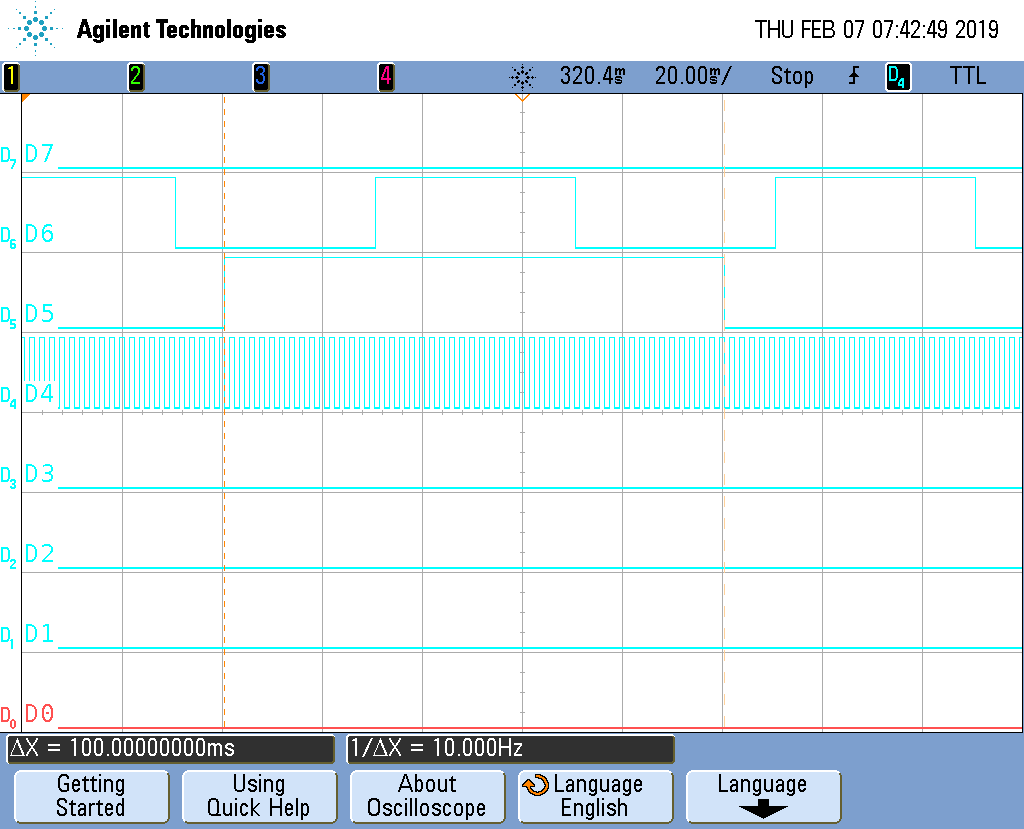
\includegraphics[width=.8\textwidth]{00.png}
\caption{The off-off, 40ms delay with button delay}
\end{figure}

\begin{figure}[htp]
\centering
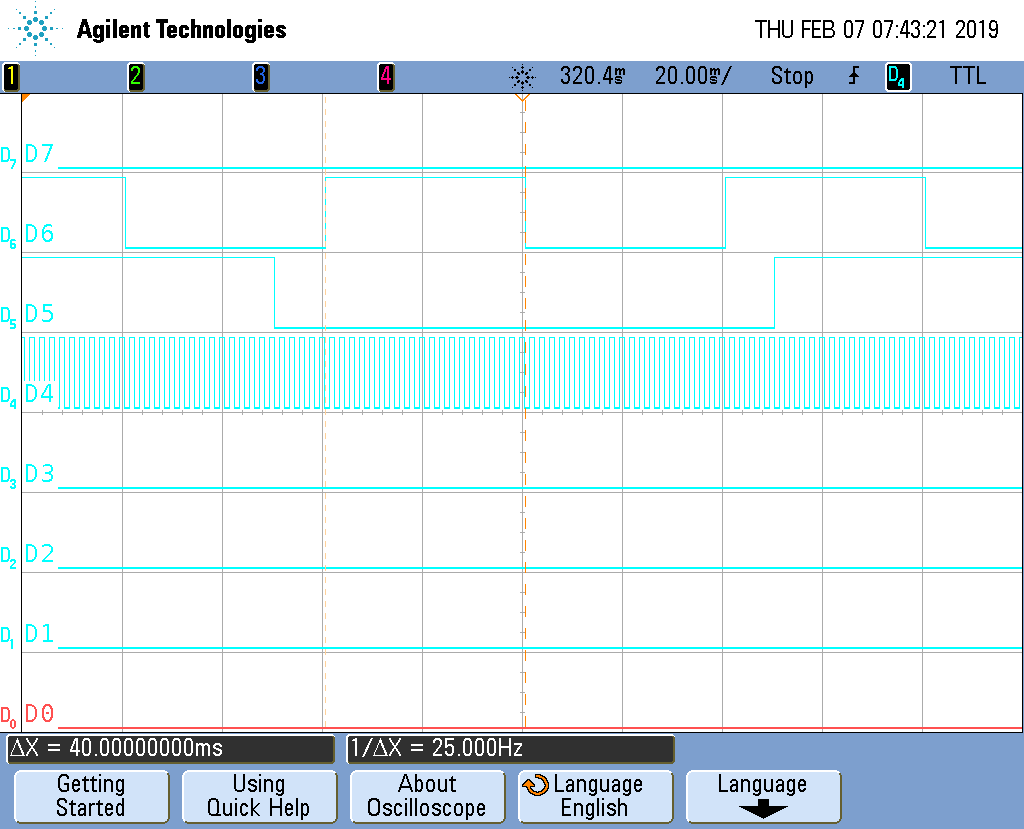
\includegraphics[width=.8\textwidth]{01.png}
\caption{The off-on 40ms delay}
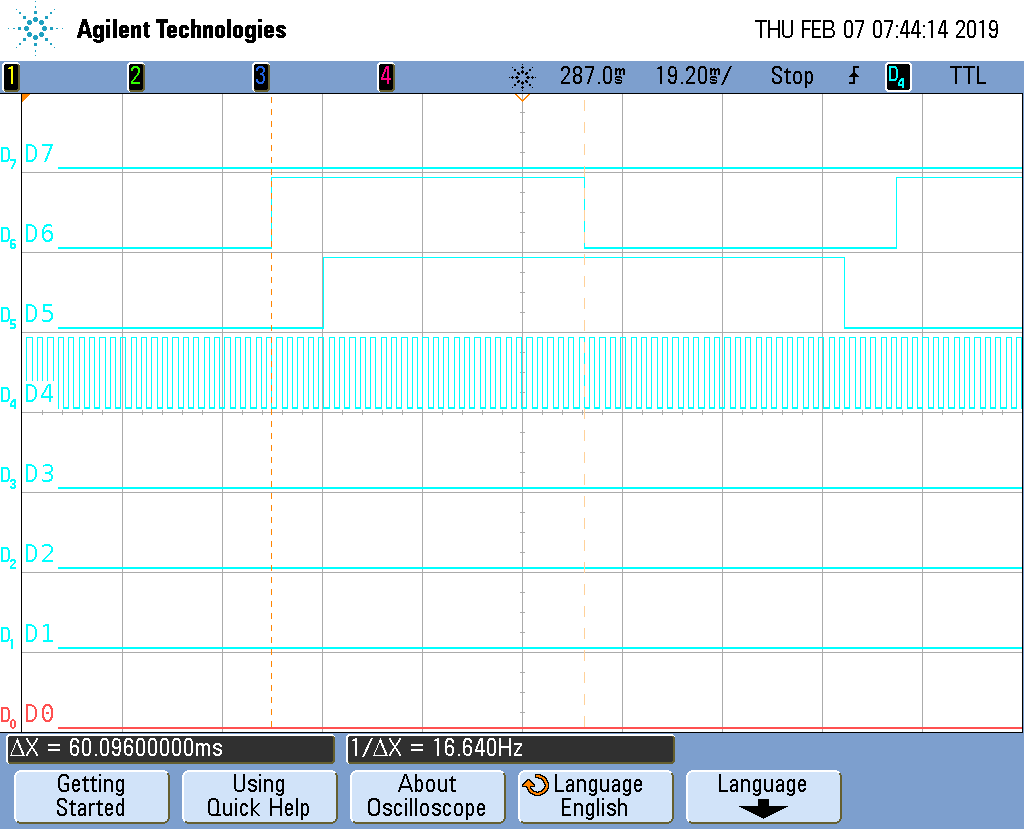
\includegraphics[width=.8\textwidth]{10.png}
\caption{The on-off 60ms delay}
\end{figure}

\begin{figure}[htb]
\centering
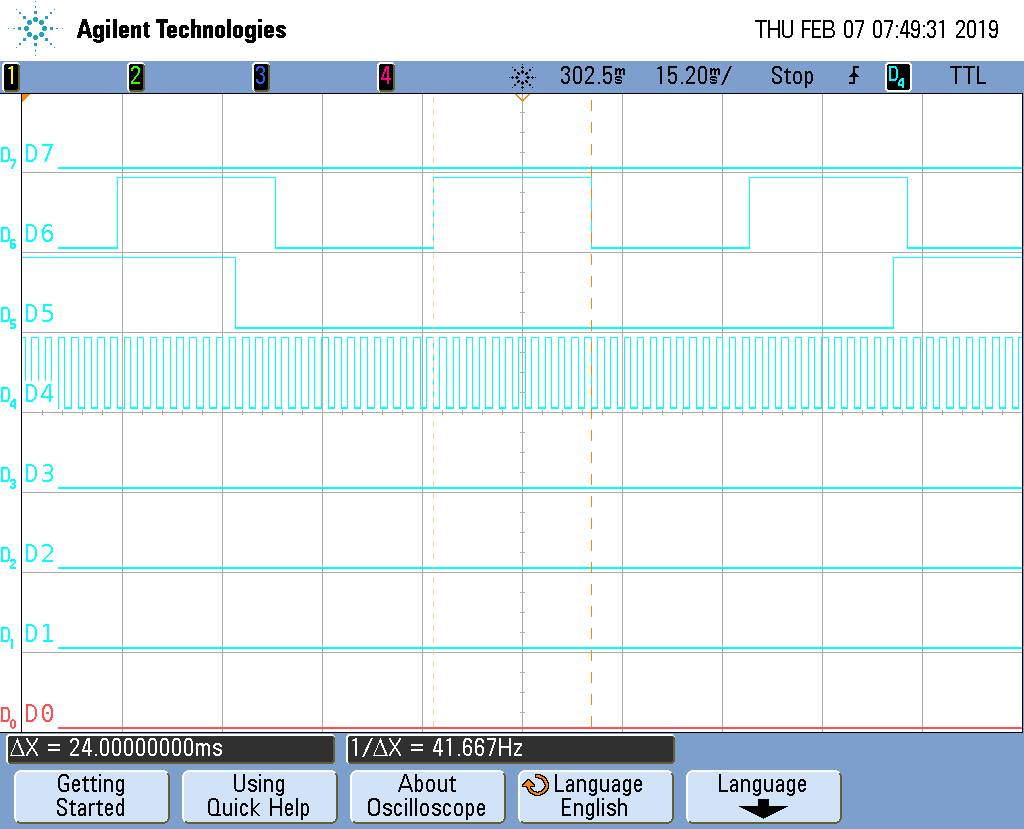
\includegraphics[width=.8\textwidth]{11.png}
\caption{The on-on 24ms delay}
\end{figure}

\end{document}